\documentclass[12pt,a4paper]{article}
\usepackage{amsmath, amssymb, geometry, booktabs, xcolor, hyperref,
            listings, pgfplots, tcolorbox, enumitem, fancyhdr, tikz, array}
\usepgfplotslibrary{fillbetween}
\geometry{margin=2.5cm}
\pgfplotsset{compat=1.18}
\tcbuselibrary{skins, breakable}

% Define custom environments
\newtcolorbox{curiositybox}[1]{colback=yellow!10, colframe=orange!80, title=#1, breakable}
\newtcolorbox{infobox}[1]{colback=blue!5, colframe=blue!60, title=#1, breakable}
\newtcolorbox{mistakebox}[1]{colback=red!5, colframe=red!60, title=#1, breakable}
\newtcolorbox{learnbox}[1]{colback=green!5, colframe=green!60, title=#1, breakable}

% Header and Footer
\pagestyle{fancy}
\fancyhf{}
\lhead{Quadratic Forms and Canonical Form}
\rhead{Unit 2 -- LAC}
\cfoot{\thepage}

% Document Title Setup
\title{\textbf{Quadratic Forms and Canonical Form} \\ \large Unit 2 -- Eigenvalues, Eigenvectors, Diagonalization and Quadratic Forms}
\author{Department of Mathematics}
\date{\today}

\begin{document}
\maketitle
\tableofcontents
\newpage

%=============================================================
\section{Real-World Engineering Hook}
%=============================================================

\begin{curiositybox}{Why Should an Engineer Care?}
Consider a steel truss bridge under load. Every joint displacement can be assembled into a vector $\mathbf{x}$, and the total strain energy stored in the structure is
\[
  U = \mathbf{x}^{\top} K \mathbf{x},
\]
where $K$ is the global \textbf{stiffness matrix} of the bridge. This expression is a \emph{quadratic form}. If $K$ is \textbf{positive definite} -- meaning $\mathbf{x}^{\top} K \mathbf{x} > 0$ for every non-zero displacement vector $\mathbf{x}$ -- the structure stores energy under any deformation and will spring back: the bridge is \textbf{stable}. If $K$ is only positive semi-definite or indefinite, certain displacement modes cost zero or negative energy, signalling a mechanism (unrestrained rigid-body motion) or an unstable mode -- the bridge collapses.

The same mathematics reappears in \textbf{Lyapunov stability analysis} of a dynamical system $\dot{\mathbf{x}} = A\mathbf{x}$. Engineers choose a candidate Lyapunov function $V(\mathbf{x}) = \mathbf{x}^{\top} P \mathbf{x}$ and verify positive definiteness of $P$ together with negative definiteness of $\dot{V}$ to certify that the closed-loop control system is globally asymptotically stable. Without quadratic-form theory, neither bridge design nor autopilot certification could be carried out rigorously. This lecture develops every tool you need.
\end{curiositybox}

%=============================================================
\section{Why This Topic Exists}
%=============================================================

\begin{center}
\begin{tabular}{@{}p{3.5cm}p{5cm}p{6cm}@{}}
\toprule
\textbf{Sub-Topic} & \textbf{Core Mathematical Idea} & \textbf{Engineering Consequence} \\
\midrule
Definition \& Matrix Form
  & Express $Q(\mathbf{x}) = \mathbf{x}^{\top}A\mathbf{x}$, symmetric $A$
  & Compact matrix notation enables finite-element assembly of stiffness matrices \\
\addlinespace
Orthogonal Reduction
  & Diagonalise $A = Q\Lambda Q^{\top}$, substitute $\mathbf{x} = Q\mathbf{y}$
  & Principal-axis transformation decouples vibrational modes of a structure \\
\addlinespace
Lagrange's Method
  & Complete the square without eigenvalues
  & Fast classification of conic sections in computer vision and robotics \\
\addlinespace
Nature of Quadratic Form
  & Classify PD, ND, PSD, NSD, Indefinite
  & Determines structural stability, convexity of cost functions in optimisation \\
\addlinespace
Rank, Index, Signature
  & Count non-zero, positive, and net eigenvalues
  & Identifies degenerate modes and redundant constraints in structural analysis \\
\bottomrule
\end{tabular}
\end{center}

\begin{learnbox}{Learning Objectives}
After studying this unit you will be able to:
\begin{itemize}[leftmargin=1.5em]
  \item Express any quadratic form in the compact matrix notation $\mathbf{x}^{\top}A\mathbf{x}$.
  \item Reduce a quadratic form to canonical form using both the orthogonal transformation method and Lagrange's method of completing the square.
  \item Classify the nature of a quadratic form using eigenvalues and Sylvester's criterion.
  \item Compute the rank, index, and signature of a quadratic form and state Sylvester's law of inertia.
  \item Apply these ideas to judge structural stability and convexity of engineering objective functions.
\end{itemize}
\end{learnbox}

%=============================================================
\section{Intuition and Mathematical Definitions}
%=============================================================

\subsection{Definition and Matrix Representation}

A quadratic form is the multi-variable generalisation of $ax^{2}$. In two variables it looks like $ax^{2} + 2hxy + by^{2}$; the cross term $2hxy$ is the only new ingredient. The key algebraic insight is that every such expression can be written as a single matrix product $\mathbf{x}^{\top}A\mathbf{x}$ where $A$ is \emph{symmetric}. Symmetry of $A$ is not a restriction -- it is a choice we make to ensure a unique representation.

\begin{infobox}{Definition: Quadratic Form and Matrix Representation}
\textbf{Quadratic form in $n$ variables:} A homogeneous polynomial of degree 2,
\[
  Q(\mathbf{x}) = \sum_{i=1}^{n}\sum_{j=1}^{n} a_{ij}\, x_i x_j
  = \mathbf{x}^{\top} A \mathbf{x}, \qquad \mathbf{x} \in \mathbb{R}^{n},
\]
where $A = (a_{ij})$ is a \textbf{real symmetric} matrix ($A = A^{\top}$).

\textbf{Two-variable form:}
$Q(x,y) = ax^{2} + 2hxy + by^{2}
= \begin{pmatrix} x & y \end{pmatrix}
  \begin{pmatrix} a & h \\ h & b \end{pmatrix}
  \begin{pmatrix} x \\ y \end{pmatrix}.$

\textbf{Three-variable form:}
$Q(x,y,z) = ax^{2}+by^{2}+cz^{2}+2fyz+2gxz+2hxy$
$= \begin{pmatrix} x & y & z \end{pmatrix}
   \begin{pmatrix} a & h & g \\ h & b & f \\ g & f & c \end{pmatrix}
   \begin{pmatrix} x \\ y \\ z \end{pmatrix}.$

\textbf{Rule for writing $A$:} The diagonal entry $a_{ii}$ is the coefficient of $x_i^{2}$; the off-diagonal entry $a_{ij} = a_{ji}$ is \emph{half} the coefficient of $x_i x_j$.
\end{infobox}

\textbf{Worked Example 3.1.1} Write $Q = 5x^{2} + 4y^{2} + 3z^{2} + 6xy - 4xz + 8yz$ in matrix form $\mathbf{x}^{\top}A\mathbf{x}$.

\textit{Solution.}
\begin{align*}
a_{11} &= 5,\quad a_{22}=4,\quad a_{33}=3,\\
a_{12} &= a_{21} = \tfrac{1}{2}(6) = 3,\quad
a_{13} = a_{31} = \tfrac{1}{2}(-4) = -2,\quad
a_{23} = a_{32} = \tfrac{1}{2}(8) = 4.
\end{align*}
Therefore
\[
  A = \begin{pmatrix} 5 & 3 & -2 \\ 3 & 4 & 4 \\ -2 & 4 & 3 \end{pmatrix}, \qquad
  Q = \begin{pmatrix} x & y & z \end{pmatrix}
      \begin{pmatrix} 5 & 3 & -2 \\ 3 & 4 & 4 \\ -2 & 4 & 3 \end{pmatrix}
      \begin{pmatrix} x \\ y \\ z \end{pmatrix}.
\]
Verification: row 1 of $A$ times $\mathbf{x}$ gives $5x+3y-2z$; multiplied by $x$ yields $5x^{2}+3xy-2xz$; adding the symmetric contribution $3yx - 2zx = 6xy - 4xz$, and continuing for rows 2 and 3 recovers $Q$ exactly. \hfill$\square$

% -----------------------------------------------------------
\subsection{Reduction to Canonical Form via Orthogonal Transformation}

Think of the level surface $Q(\mathbf{x}) = c$ as a tilted ellipse or hyperbola in the original coordinates. An orthogonal transformation rotates the axes so that they align with the principal axes of the ellipse --- the cross terms vanish and the quadratic form becomes a sum of pure squares, called the \textbf{canonical form}. The rotation matrix whose columns are eigenvectors of $A$ does this job.

\begin{infobox}{Orthogonal Reduction to Canonical Form}
\textbf{Procedure:}
\begin{enumerate}[leftmargin=1.5em]
  \item Find the eigenvalues $\lambda_1, \lambda_2, \ldots, \lambda_n$ of the symmetric matrix $A$.
  \item Find orthonormal eigenvectors $\mathbf{q}_1, \mathbf{q}_2, \ldots, \mathbf{q}_n$ corresponding to these eigenvalues.
  \item Form the orthogonal matrix $Q = [\mathbf{q}_1\; \mathbf{q}_2\;\cdots\; \mathbf{q}_n]$ (columns are eigenvectors, $Q^{\top}Q = I$, $Q^{-1}=Q^{\top}$).
  \item Substitute $\mathbf{x} = Q\mathbf{y}$: \quad
        $Q(\mathbf{x}) = \mathbf{x}^{\top}A\mathbf{x} = (Q\mathbf{y})^{\top}A(Q\mathbf{y}) = \mathbf{y}^{\top}(Q^{\top}AQ)\mathbf{y} = \mathbf{y}^{\top}\Lambda\mathbf{y}$.
  \item \textbf{Canonical form:} $Q = \lambda_1 y_1^{2} + \lambda_2 y_2^{2} + \cdots + \lambda_n y_n^{2}$.
\end{enumerate}

\textbf{Key result:} $Q^{\top}AQ = \Lambda = \mathrm{diag}(\lambda_1,\ldots,\lambda_n)$ (Spectral Theorem for real symmetric matrices).

\textbf{Principal-axis theorem:} The transformation $\mathbf{x} = Q\mathbf{y}$ is a \emph{rigid rotation}; it preserves lengths and angles, so the canonical form is equivalent to the original form under a rotation of axes.
\end{infobox}

\textbf{Worked Example 3.2.1} Reduce $Q = 2x^{2} + 3y^{2} + 2xy$ to canonical form via orthogonal transformation.

\textit{Step 1 -- Matrix form.}
Coefficient of $x^{2}$: 2; coefficient of $y^{2}$: 3; coefficient of $xy$: 2, so $a_{12}=1$.
\[
A = \begin{pmatrix} 2 & 1 \\ 1 & 3 \end{pmatrix}.
\]

\textit{Step 2 -- Eigenvalues.}
\[
\det(A - \lambda I) = (2-\lambda)(3-\lambda)-1 = \lambda^{2}-5\lambda+5=0
\implies \lambda = \frac{5 \pm \sqrt{5}}{2}.
\]
So $\lambda_1 = \dfrac{5-\sqrt{5}}{2} \approx 1.382$ and $\lambda_2 = \dfrac{5+\sqrt{5}}{2} \approx 3.618$.

\textit{Step 3 -- Eigenvectors.}
For $\lambda_1 = \frac{5-\sqrt{5}}{2}$: $(A-\lambda_1 I)\mathbf{v}=\mathbf{0}$.
Row 1: $\left(2 - \frac{5-\sqrt{5}}{2}\right)v_1 + v_2 = 0 \implies \frac{-1+\sqrt{5}}{2}v_1 + v_2 = 0$.
Choose $v_1 = 2$, $v_2 = 1-\sqrt{5}$.
Normalised: $\|\mathbf{v}_1\| = \sqrt{4+(1-\sqrt{5})^{2}} = \sqrt{4+6-2\sqrt{5}} = \sqrt{10-2\sqrt{5}}$.
$\mathbf{q}_1 = \dfrac{1}{\sqrt{10-2\sqrt{5}}}\begin{pmatrix}2\\1-\sqrt{5}\end{pmatrix}$.

For $\lambda_2 = \frac{5+\sqrt{5}}{2}$: similarly $v_1 = 2$, $v_2 = 1+\sqrt{5}$; $\|\mathbf{v}_2\|=\sqrt{10+2\sqrt{5}}$.
$\mathbf{q}_2 = \dfrac{1}{\sqrt{10+2\sqrt{5}}}\begin{pmatrix}2\\1+\sqrt{5}\end{pmatrix}$.

\textit{Step 4 -- Canonical form.}
Under $\mathbf{x} = Q\mathbf{y}$:
\[
\boxed{Q = \frac{5-\sqrt{5}}{2}\,y_1^{2} + \frac{5+\sqrt{5}}{2}\,y_2^{2}.}
\]
Both eigenvalues are positive, confirming $Q$ is positive definite. \hfill$\square$

% -----------------------------------------------------------
\subsection{Lagrange's Method of Completing the Square}

Eigenvalue computation can be tedious for large matrices. Lagrange's method provides an algebraic shortcut: group all terms containing $x_1$, complete the square, eliminate $x_1$, then repeat for $x_2$, and so on. The result is the same canonical form but obtained without solving any characteristic equation.

\begin{infobox}{Lagrange's Method: Algorithm}
\textbf{Case A -- Leading variable $x_1$ appears with non-zero coefficient $a_{11} \neq 0$:}
\begin{enumerate}[leftmargin=1.5em]
  \item Collect all terms involving $x_1$: $a_{11}x_1^{2} + 2x_1(\text{terms in }x_2,\ldots,x_n) + \text{rest}$.
  \item Complete the square: $a_{11}\!\left(x_1 + \dfrac{a_{12}x_2+\cdots+a_{1n}x_n}{a_{11}}\right)^{\!2} - \dfrac{1}{a_{11}}(a_{12}x_2+\cdots+a_{1n}x_n)^{2} + \text{rest}$.
  \item Substitute $y_1 = x_1 + \dfrac{a_{12}x_2+\cdots}{a_{11}}$ and continue with the remaining form in $x_2,\ldots,x_n$.
\end{enumerate}

\textbf{Case B -- $a_{11}=0$ but $a_{1j}\neq 0$ for some $j$:}
First apply the substitution $x_1 = u_1 + u_j$, $x_j = u_1 - u_j$ (cross-term trick) to create a non-zero leading coefficient, then apply Case A.

\textbf{Output:} Canonical form $c_1 y_1^{2} + c_2 y_2^{2} + \cdots + c_r y_r^{2}$ where $r \leq n$ and $c_i \neq 0$; the transformation $\mathbf{x} \to \mathbf{y}$ is non-singular but generally \emph{not} orthogonal.

\textbf{Note:} Different completion sequences yield different transformations but the \emph{same} set of signs among $c_i$ (Sylvester's law of inertia).
\end{infobox}

\textbf{Worked Example 3.3.1} Reduce $Q = x^{2} + 2y^{2} + z^{2} + 2xy + 2xz$ to canonical form by Lagrange's method.

\textit{Step 1 -- Collect terms in $x$.}
\[
Q = x^{2} + 2x(y+z) + 2y^{2} + z^{2}.
\]

\textit{Step 2 -- Complete the square in $x$.}
\[
Q = \bigl[x^{2} + 2x(y+z) + (y+z)^{2}\bigr] - (y+z)^{2} + 2y^{2} + z^{2}
  = (x+y+z)^{2} - y^{2} - 2yz - z^{2} + 2y^{2} + z^{2}.
\]

\textit{Step 3 -- Simplify the residual form.}
\[
-y^{2}-2yz-z^{2}+2y^{2}+z^{2} = y^{2}-2yz.
\]
So $Q = (x+y+z)^{2} + y^{2} - 2yz$.

\textit{Step 4 -- Complete the square in $y$.}
\[
y^{2} - 2yz = (y-z)^{2} - z^{2}.
\]
Hence
\[
Q = (x+y+z)^{2} + (y-z)^{2} - z^{2}.
\]

\textit{Step 5 -- Introduce canonical variables.}
Set $u_1 = x+y+z$, $u_2 = y-z$, $u_3 = z$.
\[
\boxed{Q = u_1^{2} + u_2^{2} - u_3^{2}.}
\]

\textit{Verification.} $u_1^{2}+u_2^{2}-u_3^{2} = (x+y+z)^{2}+(y-z)^{2}-z^{2}$.
Expanding: $x^{2}+y^{2}+z^{2}+2xy+2xz+2yz + y^{2}-2yz+z^{2} - z^{2}$
$= x^{2}+2y^{2}+z^{2}+2xy+2xz$ = original $Q$. \checkmark \hfill$\square$

% -----------------------------------------------------------
\subsection{Nature of Quadratic Form}

The nature of $Q$ answers the practical question: is this objective function (energy, error, cost) always positive, always negative, or mixed? The answer determines stability, convexity, and the character of extrema.

\begin{infobox}{Classification of Nature: Definitions and Criteria}
\textbf{Definitions} (let $Q = \mathbf{x}^{\top}A\mathbf{x}$, $A$ real symmetric, $\mathbf{x} \in \mathbb{R}^{n}$, $\mathbf{x}\neq\mathbf{0}$):

\begin{center}
\begin{tabular}{@{}lll@{}}
\toprule
Nature & Eigenvalue Criterion & Geometric Shape \\
\midrule
Positive Definite (PD)       & All $\lambda_i > 0$     & Ellipsoidal bowl (minimum at origin) \\
Negative Definite (ND)       & All $\lambda_i < 0$     & Inverted bowl (maximum at origin) \\
Positive Semi-Definite (PSD) & All $\lambda_i \geq 0$, at least one $= 0$ & Degenerate bowl, flat direction \\
Negative Semi-Definite (NSD) & All $\lambda_i \leq 0$, at least one $= 0$ & Inverted degenerate bowl \\
Indefinite                   & At least one $\lambda_i > 0$ and one $< 0$ & Saddle surface \\
\bottomrule
\end{tabular}
\end{center}

\textbf{Sylvester's Criterion (PD only):} $Q$ is positive definite $\iff$ all \emph{leading principal minors} $\Delta_k > 0$:
\[
  \Delta_1 = a_{11},\quad
  \Delta_2 = \begin{vmatrix} a_{11}&a_{12}\\a_{21}&a_{22}\end{vmatrix},\quad
  \Delta_3 = \begin{vmatrix} a_{11}&a_{12}&a_{13}\\a_{21}&a_{22}&a_{23}\\a_{31}&a_{32}&a_{33}\end{vmatrix}, \quad \ldots
\]

\textbf{Corollary:} $Q$ is negative definite $\iff$ $(-1)^{k}\Delta_k > 0$ for $k=1,2,\ldots,n$.
\end{infobox}

\textbf{Worked Example 3.4.1} Classify $Q = 4x^{2} + 6y^{2} + 2z^{2} - 4xy + 2xz - 4yz$ using Sylvester's criterion.

\textit{Matrix of $Q$.}
\[
A = \begin{pmatrix} 4 & -2 & 1 \\ -2 & 6 & -2 \\ 1 & -2 & 2 \end{pmatrix}.
\]

\textit{Leading principal minors.}
\[
\Delta_1 = 4 > 0.
\]
\[
\Delta_2 = \begin{vmatrix} 4 & -2 \\ -2 & 6 \end{vmatrix} = 24 - 4 = 20 > 0.
\]
\[
\Delta_3 = \det A.
\]
Expanding along row 1:
\[
\det A = 4\begin{vmatrix}6&-2\\-2&2\end{vmatrix} - (-2)\begin{vmatrix}-2&-2\\1&2\end{vmatrix} + 1\begin{vmatrix}-2&6\\1&-2\end{vmatrix}.
\]
\[
= 4(12-4) + 2(-4+2) + 1(4-6) = 4(8)+2(-2)+(-2) = 32-4-2 = 26 > 0.
\]

Since $\Delta_1 = 4 > 0$, $\Delta_2 = 20 > 0$, $\Delta_3 = 26 > 0$, Sylvester's criterion confirms $Q$ is \textbf{positive definite}. \hfill$\square$

% -----------------------------------------------------------
\subsection{Rank, Index, and Signature}

Once the canonical form is found, three integers give a complete invariant description of the quadratic form: how many squared terms survive, how many are positive, and what their net excess is. Sylvester's law of inertia guarantees these numbers are independent of which method produced the canonical form.

\begin{infobox}{Rank, Index, Signature and Sylvester's Law of Inertia}
Let $Q = c_1 y_1^{2} + c_2 y_2^{2} + \cdots + c_r y_r^{2}$ be the canonical form ($c_i \neq 0$, $r \leq n$). Define:

\begin{itemize}[leftmargin=1.5em]
  \item \textbf{Rank} $\rho$: the number of non-zero terms in the canonical form (equals rank of $A$, equals number of non-zero eigenvalues).
  \item \textbf{Index} $p$: the number of \emph{positive} coefficients $c_i$ in the canonical form (equals number of positive eigenvalues).
  \item \textbf{Signature} $s = p - q$, where $q = \rho - p$ = number of negative coefficients. Thus $s = 2p - \rho$.
\end{itemize}

\textbf{Sylvester's Law of Inertia:} Whatever non-singular linear transformation reduces $Q$ to a sum of squares, the number of positive squares $p$ and the number of negative squares $q$ are invariants (they depend only on $A$, not on the transformation chosen).

\textbf{Nature from rank/index:}
\begin{center}
\begin{tabular}{@{}lll@{}}
\toprule
$\rho$ & $p$ & Nature \\
\midrule
$n$ & $n$   & Positive Definite \\
$n$ & $0$   & Negative Definite \\
$n$ & $0<p<n$ & Indefinite \\
$r<n$ & $r$ & Positive Semi-Definite \\
$r<n$ & $0$ & Negative Semi-Definite \\
\bottomrule
\end{tabular}
\end{center}
\end{infobox}

\textbf{Worked Example 3.5.1} Find the rank, index, and signature of $Q = 3x^{2} - 5y^{2} + 2z^{2}$.

This form is already canonical (no cross terms): $c_1 = 3$, $c_2 = -5$, $c_3 = 2$.

\textit{Rank:} All three coefficients are non-zero, so $\rho = 3$.

\textit{Index:} Positive coefficients: $c_1 = 3 > 0$ and $c_3 = 2 > 0$, so $p = 2$.

\textit{Negative count:} $q = \rho - p = 3 - 2 = 1$.

\textit{Signature:} $s = p - q = 2 - 1 = 1$.

\textit{Nature:} $\rho = n = 3$ but $0 < p = 2 < 3$, so $Q$ is \textbf{indefinite}. \hfill$\square$

%=============================================================
\section{Visual Artifacts and Geometric Interpretation}
%=============================================================

\subsection*{4.1 Positive Definite vs Indefinite Quadratic Forms (3D Surface)}

\begin{center}
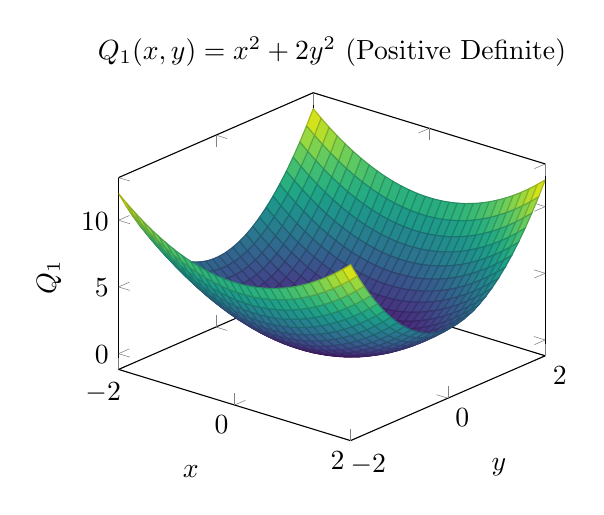
\begin{tikzpicture}
\begin{axis}[
  title={$Q_1(x,y)=x^2+2y^2$ (Positive Definite)},
  xlabel={$x$}, ylabel={$y$}, zlabel={$Q_1$},
  width=7cm, height=6cm,
  colormap/viridis,
  view={40}{30},
]
\addplot3[surf, samples=30, domain=-2:2]
  {x^2 + 2*y^2};
\end{axis}
\end{tikzpicture}
\hspace{1cm}
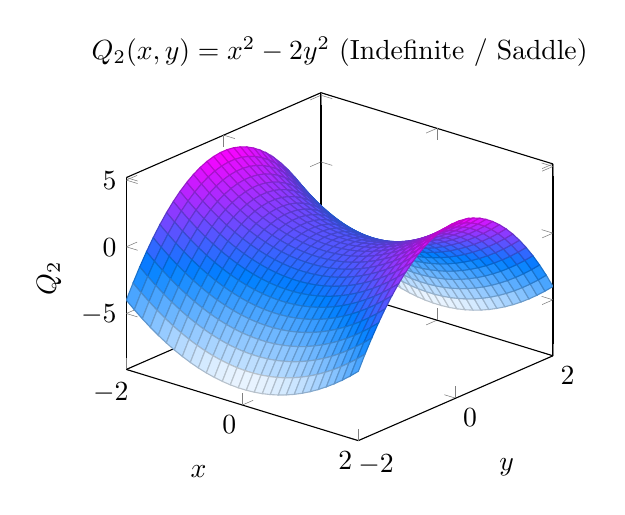
\begin{tikzpicture}
\begin{axis}[
  title={$Q_2(x,y)=x^2-2y^2$ (Indefinite / Saddle)},
  xlabel={$x$}, ylabel={$y$}, zlabel={$Q_2$},
  width=7cm, height=6cm,
  colormap/cool,
  view={40}{30},
]
\addplot3[surf, samples=30, domain=-2:2]
  {x^2 - 2*y^2};
\end{axis}
\end{tikzpicture}
\end{center}

\subsection*{4.2 Principal Axes: Orthogonal Transformation Geometry}

The diagram below illustrates how the orthogonal matrix $Q$ (whose columns are eigenvectors $\mathbf{q}_1, \mathbf{q}_2$) rotates the standard coordinate axes onto the principal axes of the ellipse $\mathbf{x}^{\top}A\mathbf{x} = 1$.

\begin{center}
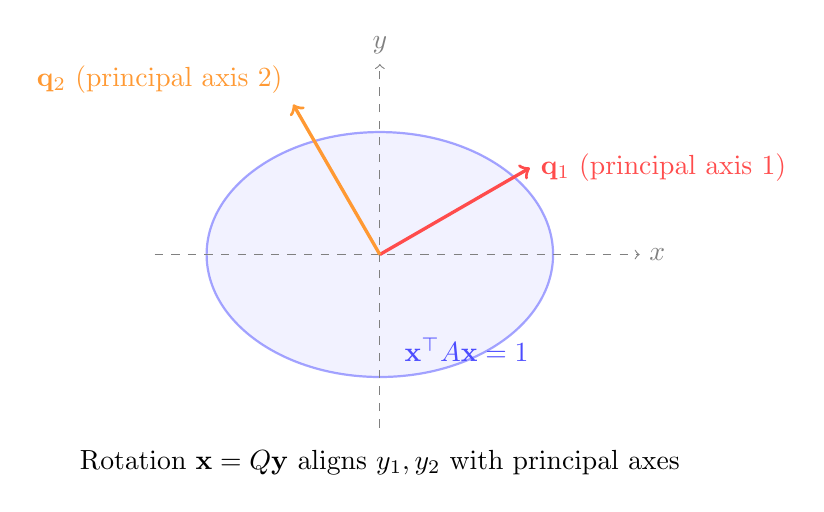
\begin{tikzpicture}[scale=2.2]
  % Draw the ellipse: semi-axes 1/sqrt(lambda1) and 1/sqrt(lambda2)
  % using lambda1=1, lambda2=2 => semi-axes 1.0 and 0.707
  \draw[thick, blue!70, fill=blue!10, opacity=0.5]
    (0,0) ellipse (1.0cm and 0.707cm);
  % Original axes (thin, dashed)
  \draw[dashed, gray, ->] (-1.3,0) -- (1.5,0) node[right] {$x$};
  \draw[dashed, gray, ->] (0,-1.0) -- (0,1.1) node[above] {$y$};
  % Rotated principal axes (eigenvectors), rotation by 30 degrees for illustration
  \draw[very thick, red!70, ->]
    (0,0) -- ({cos(30)},{sin(30)}) node[right] {$\mathbf{q}_1$ (principal axis 1)};
  \draw[very thick, orange!80, ->]
    (0,0) -- ({-sin(30)},{cos(30)}) node[above left] {$\mathbf{q}_2$ (principal axis 2)};
  % Labels
  \node[blue!70] at (0.5, -0.55) {$\mathbf{x}^{\top}A\mathbf{x}=1$};
  \node at (0,-1.2) {Rotation $\mathbf{x}=Q\mathbf{y}$ aligns $y_1,y_2$ with principal axes};
\end{tikzpicture}
\end{center}

%=============================================================
\section{Step-by-Step Algorithmic Workflow}
%=============================================================

\begin{enumerate}[label=\textbf{Step \arabic*.}, leftmargin=2.5em]
  \item \textbf{Write $Q$ in matrix form $\mathbf{x}^{\top}A\mathbf{x}$.}
    Identify diagonal entries as coefficients of pure squares; off-diagonal entries as half the coefficient of the corresponding mixed term. Verify $A = A^{\top}$.

  \item \textbf{Choose method -- Orthogonal Transformation or Lagrange.}
    \begin{itemize}[leftmargin=1.5em]
      \item Orthogonal: proceed to Steps 3--5.
      \item Lagrange: proceed to Step 6.
    \end{itemize}

  \item \textbf{(Orthogonal) Find eigenvalues of $A$.}
    Solve $\det(A - \lambda I) = 0$. For an $n\times n$ matrix this is a degree-$n$ polynomial. Record all eigenvalues $\lambda_1 \leq \lambda_2 \leq \cdots \leq \lambda_n$ (counting multiplicity).

  \item \textbf{(Orthogonal) Find orthonormal eigenvectors.}
    For each eigenvalue solve $(A-\lambda_k I)\mathbf{v} = \mathbf{0}$. If eigenvalues are repeated, use Gram-Schmidt orthogonalisation within each eigenspace. Normalise every eigenvector.

  \item \textbf{(Orthogonal) Form $Q$ (modal matrix) and write canonical form.}
    $Q = [\mathbf{q}_1 \; \cdots \; \mathbf{q}_n]$ (orthogonal). Canonical form: $\lambda_1 y_1^{2} + \cdots + \lambda_n y_n^{2}$ under $\mathbf{x} = Q\mathbf{y}$.

  \item \textbf{(Lagrange) Complete the square iteratively.}
    Start with $x_1$ (if $a_{11}\neq 0$): group all terms containing $x_1$, complete the square, set $y_1$ = completed expression, reduce the remainder by $n-1$ variables. Repeat for $x_2$, etc.

  \item \textbf{Classify the nature.}
    \begin{itemize}[leftmargin=1.5em]
      \item All canonical coefficients (or eigenvalues) $> 0$: Positive Definite.
      \item All $< 0$: Negative Definite.
      \item Mix of signs: Indefinite.
      \item All $\geq 0$ with at least one $= 0$: Positive Semi-Definite.
      \item All $\leq 0$ with at least one $= 0$: Negative Semi-Definite.
    \end{itemize}

  \item \textbf{Read off rank, index, signature.}
    $\rho$ = number of non-zero canonical coefficients; $p$ = number of positive; $s = p - (\rho - p) = 2p - \rho$.
\end{enumerate}

%=============================================================
\section{Fully Worked Step-by-Step Numerical Examples}
%=============================================================

\subsection*{Example 6.1 -- Matrix Form and Canonical Form via Eigenvalues}

Reduce $Q = 2x^{2} + 3y^{2} + 2xy$ to canonical form via the orthogonal transformation method.

\textbf{Matrix form.}
\[
A = \begin{pmatrix} 2 & 1 \\ 1 & 3 \end{pmatrix}.
\]

\textbf{Characteristic equation.}
\[
\det(A - \lambda I)
= (2-\lambda)(3-\lambda)-1
= \lambda^{2} - 5\lambda + 5 = 0.
\]
\[
\lambda = \frac{5 \pm \sqrt{25-20}}{2} = \frac{5 \pm \sqrt{5}}{2}.
\]
$\lambda_1 = \dfrac{5-\sqrt{5}}{2}$,\quad $\lambda_2 = \dfrac{5+\sqrt{5}}{2}$.

\textbf{Eigenvectors.}
For $\lambda_1$: $(2 - \lambda_1)v_1 + v_2 = 0 \implies v_2 = (\lambda_1 - 2)v_1 = \dfrac{\sqrt{5}-1}{2}v_1$.
Set $v_1 = 2$: $v_2 = \sqrt{5}-1$.
$\|\mathbf{v}_1\|^{2} = 4 + (\sqrt{5}-1)^{2} = 4 + 6 - 2\sqrt{5} = 10 - 2\sqrt{5}$.
$\mathbf{q}_1 = \dfrac{1}{\sqrt{10-2\sqrt{5}}}\begin{pmatrix}2\\\sqrt{5}-1\end{pmatrix}$.

For $\lambda_2$: $v_2 = -(\sqrt{5}+1)/2 \cdot (-2)$ ... similarly $\mathbf{q}_2 = \dfrac{1}{\sqrt{10+2\sqrt{5}}}\begin{pmatrix}2\\-(\sqrt{5}+1)\end{pmatrix}$.

\textbf{Canonical form} (under $\mathbf{x} = Q\mathbf{y}$):
\[
\boxed{Q = \frac{5-\sqrt{5}}{2}\,y_1^{2} + \frac{5+\sqrt{5}}{2}\,y_2^{2}.}
\]
Both eigenvalues are positive ($\lambda_1 \approx 1.382 > 0$, $\lambda_2 \approx 3.618 > 0$): \textbf{Positive Definite}.
Rank $= 2$, Index $= 2$, Signature $= 2 - 0 = 2$. \hfill$\square$

\subsection*{Example 6.2 -- Lagrange's Method}

Reduce $Q = x^{2} + 2y^{2} + z^{2} + 2xy + 2xz$ to canonical form using Lagrange's method.

\textbf{Step 1.} Group terms in $x$: $Q = x^{2} + 2x(y+z) + 2y^{2} + z^{2}$.

\textbf{Step 2.} Add and subtract $(y+z)^{2}$:
\[
Q = [x^{2} + 2x(y+z) + (y+z)^{2}] - (y+z)^{2} + 2y^{2} + z^{2}
  = (x+y+z)^{2} + R_1.
\]
\[
R_1 = -(y^{2}+2yz+z^{2}) + 2y^{2} + z^{2} = y^{2} - 2yz.
\]

\textbf{Step 3.} Complete the square in $y$ within $R_1$:
\[
R_1 = y^{2} - 2yz = (y-z)^{2} - z^{2}.
\]

\textbf{Step 4.} Canonical form with $u_1 = x+y+z$, $u_2 = y-z$, $u_3 = z$:
\[
\boxed{Q = u_1^{2} + u_2^{2} - u_3^{2}.}
\]
Rank $= 3$, Index $= 2$ (two positive coefficients), Signature $= 2-1 = 1$. Form is \textbf{indefinite}.

Verification: $(x+y+z)^{2}+(y-z)^{2}-z^{2} = x^{2}+y^{2}+z^{2}+2xy+2xz+2yz + y^{2}-2yz+z^{2}-z^{2}$
$= x^{2}+2y^{2}+z^{2}+2xy+2xz$ = original $Q$. \checkmark \hfill$\square$

\subsection*{Example 6.3 -- Engineering: Positive Definiteness via Sylvester's Criterion}

A two-degree-of-freedom structural system has stiffness matrix
\[
K = \begin{pmatrix} 6 & -2 & 1 \\ -2 & 5 & -1 \\ 1 & -1 & 3 \end{pmatrix}.
\]
Determine whether the strain energy $U = \mathbf{x}^{\top}K\mathbf{x}$ is positive definite, i.e., whether the structure is stable.

\textbf{Leading principal minors:}
\[
\Delta_1 = 6 > 0.
\]
\[
\Delta_2 = \begin{vmatrix}6&-2\\-2&5\end{vmatrix} = 30 - 4 = 26 > 0.
\]
\[
\Delta_3 = \det K.
\]
Expanding along row 1:
\[
\det K = 6\begin{vmatrix}5&-1\\-1&3\end{vmatrix}
        - (-2)\begin{vmatrix}-2&-1\\1&3\end{vmatrix}
        + 1\begin{vmatrix}-2&5\\1&-1\end{vmatrix}.
\]
\[
= 6(15-1) + 2(-6+1) + 1(2-5)
= 6(14) + 2(-5) + (-3)
= 84 - 10 - 3 = 71 > 0.
\]

Since $\Delta_1 = 6 > 0$, $\Delta_2 = 26 > 0$, $\Delta_3 = 71 > 0$, Sylvester's criterion is satisfied: $K$ is \textbf{positive definite}. The strain energy $U > 0$ for any non-zero displacement vector $\mathbf{x}$; the structure is \textbf{stable}. \hfill$\square$

%=============================================================
\section{Tabular Reference: Method Comparison}
%=============================================================

\begin{center}
\begin{tabular}{@{}p{3cm}p{4.5cm}p{4.5cm}@{}}
\toprule
\textbf{Feature} & \textbf{Orthogonal Transformation} & \textbf{Lagrange's Method} \\
\midrule
Core tool & Eigenvalue decomposition $A = Q\Lambda Q^{\top}$ & Successive completion of squares \\
\addlinespace
Transformation & Orthogonal ($Q^{-1}=Q^{\top}$, preserves lengths) & Non-singular but generally non-orthogonal \\
\addlinespace
Steps & Solve char.\ poly.\ $\to$ eigenvectors $\to$ normalise $\to$ form $Q$ & Group terms $\to$ complete square $\to$ substitute $\to$ repeat \\
\addlinespace
Canonical form output & $\sum \lambda_i y_i^{2}$ (eigenvalues as coefficients) & $\sum c_i y_i^{2}$ (arbitrary non-zero $c_i$) \\
\addlinespace
Geometric meaning & Rigid rotation to principal axes & Non-rigid shear/stretch change of variables \\
\addlinespace
Advantage & Gives principal axes, eigenvalues, geometric insight & Faster arithmetic; no eigenvalue polynomial \\
\addlinespace
Disadvantage & Requires solving degree-$n$ polynomial & Transformation is not orthogonal; harder to invert \\
\addlinespace
Invariants preserved & Rank, index, signature (Sylvester's law) & Rank, index, signature (Sylvester's law) \\
\addlinespace
Preferred when & Geometric interpretation needed; vibration modes & Quick classification without eigenvalues \\
\bottomrule
\end{tabular}
\end{center}

%=============================================================
\section{Common Student Mistakes and Pitfalls}
%=============================================================

\begin{mistakebox}{Frequent Errors in Quadratic Form Problems}
\begin{tabular}{@{}p{3.5cm}p{5.5cm}p{5.5cm}@{}}
\toprule
\textbf{Sub-Topic} & \textbf{Typical Mistake} & \textbf{Correct Practice} \\
\midrule
Definition \& Matrix Form
  & Putting the full cross-term coefficient in both $a_{ij}$ and $a_{ji}$; e.g., writing $a_{12}=a_{21}=2h$ instead of $h$
  & Always halve the cross-term coefficient: $a_{ij} = a_{ji} = \frac{1}{2}\times(\text{coeff of } x_ix_j)$ \\
\addlinespace
Orthogonal Reduction
  & Forming $Q$ with un-normalised eigenvectors, so $Q^{\top}Q \neq I$ and $Q^{\top}AQ \neq \Lambda$
  & Normalise every eigenvector to unit length before assembling the modal matrix \\
\addlinespace
Lagrange's Method
  & Forgetting to subtract the square that was added when completing; e.g., writing $(x+y)^{2}$ without subtracting $y^{2}$
  & Write $x^{2}+2xy = (x+y)^{2} - y^{2}$ and carry the $-y^{2}$ into the residual \\
\addlinespace
Nature Classification
  & Checking only the sign of the determinant of $A$ and concluding PD; $\det A > 0$ is necessary but not sufficient
  & Verify \emph{all} leading principal minors $\Delta_k > 0$ (Sylvester's criterion), or check all eigenvalues \\
\addlinespace
Rank, Index, Signature
  & Confusing index $p$ with rank $\rho$; writing signature as $p$ instead of $p - q = 2p - \rho$
  & Signature $s = p - q$ where $q$ = number of negative squares; compute $q = \rho - p$ first \\
\bottomrule
\end{tabular}
\end{mistakebox}

%=============================================================
\section{Comprehensive Assessment Suite}
%=============================================================

\subsection*{9.1 Viva-Voce Questions}

\begin{enumerate}[leftmargin=2em, label=\textbf{V\arabic*.}]
  \item \textbf{(Sub-topic 1)} What is the matrix of the quadratic form $Q = x^{2} + 4xy + 3y^{2}$? Why must this matrix be symmetric, and how do you ensure symmetry when multiple cross terms are present?

  \item \textbf{(Sub-topic 2)} Explain why the orthogonal matrix used to diagonalise a real symmetric matrix satisfies $Q^{-1} = Q^{\top}$. How does this property simplify the expression $\mathbf{x}^{\top}A\mathbf{x}$ after the substitution $\mathbf{x} = Q\mathbf{y}$?

  \item \textbf{(Sub-topic 3)} In Lagrange's method, what adjustment must you make when the leading diagonal entry $a_{11} = 0$ but there is a non-zero cross term $2a_{12}x_1x_2$? Justify why a substitution of the form $x_1 = u+v$, $x_2 = u-v$ is appropriate.

  \item \textbf{(Sub-topic 4)} A quadratic form has eigenvalues $\lambda_1 = 2$, $\lambda_2 = 0$, $\lambda_3 = -1$. What is the nature of this form? Can Sylvester's criterion be applied to check positive definiteness here? Why or why not?

  \item \textbf{(Sub-topic 5)} State Sylvester's law of inertia. Give an example showing that two different non-singular linear transformations can reduce the same quadratic form to different-looking canonical forms, yet the number of positive and negative squares remains the same.

  \item \textbf{(Sub-topic 1 \& 4)} If the stiffness matrix $K$ of a structure is positive definite, what does this imply about the strain energy $U = \mathbf{x}^{\top}K\mathbf{x}$ for every non-zero displacement vector $\mathbf{x}$? Why is this a stability criterion?

  \item \textbf{(Sub-topic 3)} Is the transformation produced by Lagrange's method always orthogonal? If not, what property does it have, and does that affect the canonical form obtained?

  \item \textbf{(Sub-topic 5)} How is the rank of a quadratic form related to the rank of its matrix? Can a quadratic form in three variables have rank 2? Give a concrete example.
\end{enumerate}

\subsection*{9.2 Descriptive Exam Questions}

\begin{enumerate}[leftmargin=2em, label=\textbf{D\arabic*.}]
  \item Reduce the quadratic form $Q = 3x^{2} + 5y^{2} + 3z^{2} - 2yz + 2xz - 2xy$ to canonical form by an orthogonal transformation. State the nature of the form, and find its rank, index, and signature. \\
  \textit{Hint:} The matrix is $A = \begin{pmatrix}3&-1&1\\-1&5&-1\\1&-1&3\end{pmatrix}$; eigenvalues are $2, 3, 6$.

  \item Using Lagrange's method of completing the square, reduce $Q = 2x^{2} + y^{2} + 3z^{2} + 2xy - 4xz - 2yz$ to canonical form. Find the transformation used and verify by substituting back. \\
  \textit{Hint:} First complete the square in $x$, then in $y$.

  \item A control engineer models the Lyapunov function as $V(\mathbf{x}) = \mathbf{x}^{\top}P\mathbf{x}$ where
  $P = \begin{pmatrix}4&1\\1&3\end{pmatrix}$.
  Using Sylvester's criterion, verify that $V$ is positive definite, and find the canonical form via eigenvalues. State how positive definiteness of $V$ contributes to stability certification.

  \item For the quadratic form $Q = ax^{2} + 4xy + ay^{2}$, determine the values of $a$ for which $Q$ is (i) positive definite, (ii) negative definite, (iii) indefinite. Explain your reasoning using both eigenvalue analysis and Sylvester's criterion.

  \item State and prove Sylvester's law of inertia for quadratic forms over $\mathbb{R}$. Illustrate with the quadratic form $Q = x^{2} - y^{2}$ that two different non-singular transformations yield canonical forms with the same number of positive and negative squares.
\end{enumerate}

\subsection*{9.3 Multiple Choice Questions}

\begin{enumerate}[leftmargin=2em, label=\textbf{MCQ\arabic*.}]
  \item \textbf{(Sub-topic 1)} The matrix of the quadratic form $Q = x^{2} + 6xy + 2y^{2}$ is:

  (a) $\begin{pmatrix}1&6\\6&2\end{pmatrix}$
  \quad (b) $\begin{pmatrix}1&3\\3&2\end{pmatrix}$
  \quad (c) $\begin{pmatrix}1&6\\0&2\end{pmatrix}$
  \quad (d) $\begin{pmatrix}2&3\\3&1\end{pmatrix}$

  \textbf{Correct answer: (b).} Off-diagonal entries are half the coefficient of $xy$: $a_{12} = a_{21} = 3$.

  \item \textbf{(Sub-topic 2)} After the orthogonal substitution $\mathbf{x} = Q\mathbf{y}$ that diagonalises $A$, the canonical form of $\mathbf{x}^{\top}A\mathbf{x}$ is:

  (a) $\mathbf{y}^{\top}\mathbf{y}$
  \quad (b) $\mathbf{y}^{\top}A\mathbf{y}$
  \quad \textbf{(c) $\mathbf{y}^{\top}\Lambda\mathbf{y}$}
  \quad (d) $\mathbf{x}^{\top}\Lambda\mathbf{x}$

  \textbf{Correct answer: (c).} $Q^{\top}AQ = \Lambda$ (diagonal eigenvalue matrix), so the form becomes $\sum \lambda_i y_i^{2}$.

  \item \textbf{(Sub-topic 3)} In Lagrange's method, when the coefficient of $x_1^{2}$ is zero but the coefficient of $x_1 x_2$ is non-zero, the first step is to:

  (a) Swap the labels of $x_1$ and $x_2$
  \quad (b) Set $x_1 = 0$
  \quad \textbf{(c) Substitute $x_1 = u+v$, $x_2 = u-v$}
  \quad (d) Differentiate $Q$ with respect to $x_1$

  \textbf{Correct answer: (c).} This substitution creates the term $(u+v)(u-v) = u^{2}-v^{2}$, giving non-zero $u^{2}$ coefficient to proceed with completing the square.

  \item \textbf{(Sub-topic 4)} A quadratic form is positive definite if and only if:

  \textbf{(a) All eigenvalues of its matrix are strictly positive}
  \quad (b) The trace of its matrix is positive
  \quad (c) The determinant of its matrix is positive
  \quad (d) It has full rank

  \textbf{Correct answer: (a).} Positive determinant or positive trace are each necessary but not sufficient; only all-positive eigenvalues (equivalently, all positive leading principal minors) guarantee positive definiteness.

  \item \textbf{(Sub-topic 5)} If a quadratic form in 4 variables has rank 3 and index 2, its signature is:

  (a) $3$ \quad \textbf{(b) $1$} \quad (c) $-1$ \quad (d) $2$

  \textbf{Correct answer: (b).} $q = \rho - p = 3-2=1$; signature $= p - q = 2-1 = 1$.

  \item \textbf{(Sub-topic 1 \& 4)} The quadratic form $Q = x^{2} + y^{2} + z^{2} - 2xy - 2yz - 2xz$ has determinant of its matrix equal to $-4$. Its nature is:

  (a) Positive Definite \quad (b) Negative Definite \quad (c) Positive Semi-Definite \quad \textbf{(d) Indefinite}

  \textbf{Correct answer: (d).} A negative determinant means at least one eigenvalue is negative and at least one positive (since for $3\times3$, $\det A = \lambda_1\lambda_2\lambda_3 < 0$ implies an odd number of negative eigenvalues; combined with $\mathrm{tr}A = 3 > 0$, not all eigenvalues share the same sign), so the form is indefinite.
\end{enumerate}

%=============================================================
\section{Quick Recap and Formula Sheet}
%=============================================================

\begin{learnbox}{Key Formulas and Results: Quadratic Forms and Canonical Form}
\begin{itemize}[leftmargin=1.5em]
  \item \textbf{Matrix form:} $Q(\mathbf{x}) = \mathbf{x}^{\top}A\mathbf{x}$ where $A$ is real symmetric; diagonal entry $a_{ii}$ = coefficient of $x_i^{2}$; off-diagonal $a_{ij} = \frac{1}{2}\times$(coefficient of $x_ix_j$).

  \item \textbf{Canonical form via eigenvalues:} Factorise $A = Q\Lambda Q^{\top}$ (orthogonal $Q$); substitute $\mathbf{x} = Q\mathbf{y}$; canonical form $= \lambda_1 y_1^{2}+\cdots+\lambda_n y_n^{2}$.

  \item \textbf{Lagrange's method:} Complete the square in $x_1$, set $y_1 = x_1 + (\text{linear in }x_2,\ldots)$; repeat for $x_2$; output is $c_1y_1^{2}+c_2y_2^{2}+\cdots$ (non-orthogonal transformation).

  \item \textbf{Nature classification:} All eigenvalues $>0 \Rightarrow$ PD; all $<0 \Rightarrow$ ND; mixed signs $\Rightarrow$ Indefinite; all $\geq0$ with zero $\Rightarrow$ PSD; all $\leq0$ with zero $\Rightarrow$ NSD.

  \item \textbf{Sylvester's criterion (PD):} $Q$ is positive definite $\iff$ $\Delta_1>0, \Delta_2>0, \ldots, \Delta_n>0$ (all leading principal minors positive).

  \item \textbf{Rank, index, signature:} $\rho$ = non-zero canonical coefficients; $p$ = positive; $q = \rho - p$ = negative; \textbf{signature} $s = p - q = 2p - \rho$.

  \item \textbf{Sylvester's law of inertia:} The numbers $p$ and $q$ are invariants of $Q$ --- independent of which non-singular linear transformation produces the canonical form.

  \item \textbf{Engineering link:} Stiffness matrix $K$ PD $\Leftrightarrow$ all strain energy $U = \mathbf{x}^{\top}K\mathbf{x} > 0$ $\Leftrightarrow$ structural stability; Lyapunov function $V = \mathbf{x}^{\top}P\mathbf{x}$ requires $P$ PD for stability certificate.
\end{itemize}
\end{learnbox}

\end{document}
